%----------------------------------------------------------------------------------------
%    PACKAGES AND THEMES
%----------------------------------------------------------------------------------------

\documentclass[aspectratio=169,xcolor=dvipsnames]{beamer}
\usetheme{SimplePlus}

\usepackage[brazil]{babel}
\usepackage{csquotes}
\usepackage[backend=biber,style=chem-rsc,sorting=none,url=false,eprint=false,doi=false,isbn=false]{biblatex}

\usepackage{hyperref}
\usepackage{graphicx} % Allows including images
\usepackage{booktabs} % Allows the use of \toprule, \midrule and \bottomrule in tables

\usepackage{slashed}

\addbibresource{refs.bib}

\newcommand{\tgreen}[1]{\textcolor{green}{#1}}
\newcommand{\tred}[1]{\textcolor{red}{#1}}
\newcommand{\tblue}[1]{\textcolor{blue}{#1}}

\newcommand{\bm}[1]{\mathbf{#1}}

% \renewcommand{\footnotesize}{\tiny}

%----------------------------------------------------------------------------------------
%    TITLE PAGE
%----------------------------------------------------------------------------------------

\title{Métodos machine learning aplicados em estrelas de nêutrons}

\author{André G. da Silva \\ Orientador: Ricardo L. S. Farias}

\institute
{
    Departamento de Física \\
    Universidade Federal de Santa Maria % Your institution for the title page
}
\date{25 de setembro de 2025} % Date, can be changed to a custom date

%----------------------------------------------------------------------------------------
%    PRESENTATION SLIDES
%----------------------------------------------------------------------------------------

\begin{document}

\begin{frame}
	% Print the title page as the first slide
	\titlepage
\end{frame}

\begin{frame}{Conteúdo}
	\tableofcontents
\end{frame}

\section{Introdução}
\begin{frame}{Introdução}
	\begin{itemize}
		\item A cromodinâmica quântica (\tred{Q}\tgreen{C}\tblue{D}) como a teoria da interação forte;
		\item Liberdade assintótica e simetria quiral;
	\end{itemize}

	\begin{figure}
		\centering
		\includegraphics[width=0.4\textwidth]{uud.png}
		\includegraphics[width=0.4\textwidth]{proton.png}
	\end{figure}
\end{frame}

\begin{frame}
	\begin{itemize}
		\item Regimes extremos;
		\item Diagrama de fases;
		\item Equação de estado da matéria densa;
	\end{itemize}
	\begin{figure}
		\centering
		\includegraphics[width=0.47\textwidth]{QCDPD_nB.png}
		% \includegraphics[width=0.4\textwidth]{diagrama_fase_qcd.png}
		% \caption{\textbf{(Esquerda)} imagem de \fullcite{MUSES_2023}. \textbf{(Direita)} imagem de \fullcite{Aarts_2015}.}
		\caption{Regiões acessíveis por meio de experimentos e simulações. Imagem de \fullcite{MUSES_2023}.}
	\end{figure}
\end{frame}

\begin{frame}
	% \begin{itemize}
	% \item Por que obter a equação de estado de estrelas de nêutrons?
	% \end{itemize}

	\begin{center}
		\huge \textbf{Por que obter a equação de estado de estrelas de nêutrons?}
	\end{center}

	\vspace{0.5cm}

	\begin{minipage}{1.0\textwidth}
		\begin{minipage}{0.4\textwidth}
			\begin{figure}
				\centering
				\includegraphics[width=1.0\textwidth]{question.png}
			\end{figure}
		\end{minipage}
		\begin{minipage}{0.6\textwidth}
			% \begin{itemize}
		\end{minipage}
	\end{minipage}
\end{frame}

\begin{frame}[noframenumbering]
	% \begin{itemize}
	% \item Por que obter a equação de estado de estrelas de nêutrons?
	% \end{itemize}

	\begin{center}
		\huge \textbf{Por que obter a equação de estado de estrelas de nêutrons?}
	\end{center}

	\vspace{0.5cm}

	\begin{minipage}{1.0\textwidth}
		\begin{minipage}{0.4\textwidth}
			\begin{figure}
				\centering
				\includegraphics[width=1.0\textwidth]{question.png}
			\end{figure}
		\end{minipage}
		\begin{minipage}{0.6\textwidth}
			\begin{itemize}
				\item Exclusão de modelos que não descrevem a equação de estado;
				\item Ajuste de parâmetros de modelos;
				\item Fornecimento da EoS para simulações como, por exemplo, mergers de estrelas de nêutrons;
			\end{itemize}
		\end{minipage}
	\end{minipage}
\end{frame}

\begin{frame}{Quantificação de incertezas}
	\begin{itemize}
		\item Incertezas com análises Bayesianas;
	\end{itemize}
	\begin{figure}
		\centering
		\includegraphics[width=0.4\textwidth]{landry.pdf}
		\includegraphics[width=0.4\textwidth]{brandes_seg.pdf}

		\caption{\textbf{(Esquerda)} resultados de \fullcite{Landry_2020}, CIs de $90\%$. \textbf{(Direita)} resultados de \fullcite{Brandes_2023}, CIs de $68\%$ (bandas escuras) e $95\%$ (bandas claras).}
	\end{figure}
\end{frame}

\begin{frame}
	\begin{itemize}
		\item Incertezas com redes neurais;
	\end{itemize}

	\begin{figure}
		\centering

		\includegraphics[width=0.4\textwidth]{fujimoto.pdf}
		\includegraphics[width=0.4\textwidth]{soma.pdf}
		\caption{\textbf{(Esquerda)} resultados de \fullcite{Fujimoto_2024}, utilizando médias e desvios padrão. \textbf{(Direita)} resultados de \fullcite{Soma_2023}, CIs de $90\%$.}
	\end{figure}
\end{frame}

\section{Objetivos}
\begin{frame}{Objetivos}
	\begin{itemize}
		\item Desenvolver um processo de inferência da equação de estado baseado em uma forma paramétrica;
		\item Desenvolver os modelos de inferência com base em rede neural e análise Bayesiana;
		\item Quantificar as incertezas relacionadas ao processo de inversão;
		\item Obtenção da equação de estado de matéria densa, juntamente com o diagrama massa-raio associado
	\end{itemize}
\end{frame}

\section{Estrelas de nêutrons}
\begin{frame}{Estrelas de Nêutrons}
	\begin{itemize}
		\item Um dos objetos mais densos conhecidos;
		\item Rotações e campos magnéticos altos;
		\item Temperaturas baixas;
	\end{itemize}

	\begin{figure}
		\centering
		\includegraphics[width=0.8\textwidth]{neutron_star_sm.png}
	\end{figure}
\end{frame}

\begin{frame}
	\begin{figure}
		\centering
		\includegraphics[width=0.5\textwidth]{NS.png}
		\caption{Seções de uma estrela de nêutrons. Imagem de \fullcite{MUSES_2023}.}
	\end{figure}
\end{frame}

\begin{frame}
	\begin{itemize}
		\item Dados mais recentes do NICER e LIGO/Virgo;
	\end{itemize}

	\begin{figure}
		\centering

		\includegraphics[width=0.5\textwidth]{fig_mr_data.pdf}
		\caption{Compilação de medidas massa-raio medidas. Imagem de \fullcite{Fujimoto_2024}.}
	\end{figure}
\end{frame}

\begin{frame}{Equilíbrio hidrostático}
	Observações de massa e raio podem ser ligadas à equação de estado (calculada por modelos de QCD) via as equações de Tolman-Oppenheimer-Volkoff\footnote{Aqui são utilizadas unidades em que $c = 1$}:

	\begin{equation}
		\begin{aligned}
			\frac{dp}{dr} & = -\frac{\left[p(r) + \epsilon(r)\right] \left[G m(r) + 4\pi G r^3 p(r) \right]}{r \left[ r - 2G m(r) \right]}, \\
			\frac{dm}{dr} & = 4\pi r^2 \epsilon(r),
		\end{aligned}
	\end{equation}
	onde resta uma incógnita $\epsilon(r)$ que pode ser colocada na forma $\epsilon(p)$ e é chamada de equação de estado (EoS). A EoS pode ser determinada por um modelo de física nuclear ou de forma paramétrica.

\end{frame}

\begin{frame}
	Na prática, as equações de TOV proporcionam soluções em que a pressão tende lentamente a zero. Para obter raios finitos, é necessário definir uma pressão de corte $p(r = R) \sim 1\times 10^{-8} \text{[u.p.]}$, que pode depender fortemente da EoS utilizada. As equações de TOV podem ser colocadas na forma de pseudo-entalpia,

	\begin{equation}
		\begin{aligned}
			\frac{dr}{dh} & = -\frac{r(r - 2m)}{m + 4\pi r^3p(h)},                      \\
			\frac{dm}{dh} & = -\frac{4\pi \epsilon(h) r^3 (r - 2m)}{m + 4\pi r^3 p(h)},
		\end{aligned}
	\end{equation}
	onde a $h$ é dado por
	\begin{equation}
		h(p) = \int_0^p \frac{dp'}{\epsilon(p') + p'}.
	\end{equation}
\end{frame}

\begin{frame}
	Essas equações foram apresentadas originalmente por \footfullcite{Tolman_1939}$^{,}$\footfullcite{Oppenheimer_1939} e foram resolvidas para um gás de fermions degenerados. A equação de estado toma a forma\footfullcite{Sagert_2006}

	\begin{equation}
		\begin{aligned}
			\epsilon(x) & = \frac{\epsilon_n}{8} \left[ (2x^3 + x)(1 + x^2)^{\frac{1}{2}} - \sinh^{-1}(x) \right],                              \\
			p(x)        & = \frac{\epsilon_n}{24} \left[ (2x^3 - 3x)(1 + x^2)^{\frac{1}{2}} + 3\sinh^{-1}(x) \right], \quad x = \frac{k_F}{m_n}
		\end{aligned}
	\end{equation}
\end{frame}

\begin{frame}
	\begin{figure}
		\centering
		\includegraphics[width=0.45\textwidth]{fermigas_pressure.png}
		\includegraphics[width=0.45\textwidth]{fermigas_mass.png}
		\caption{Solução das equações de TOV para $p(r = 0) = 100 \; \text{MeV fm}^{-3}$.}
	\end{figure}
\end{frame}

\begin{frame}
	\begin{figure}
		\centering
		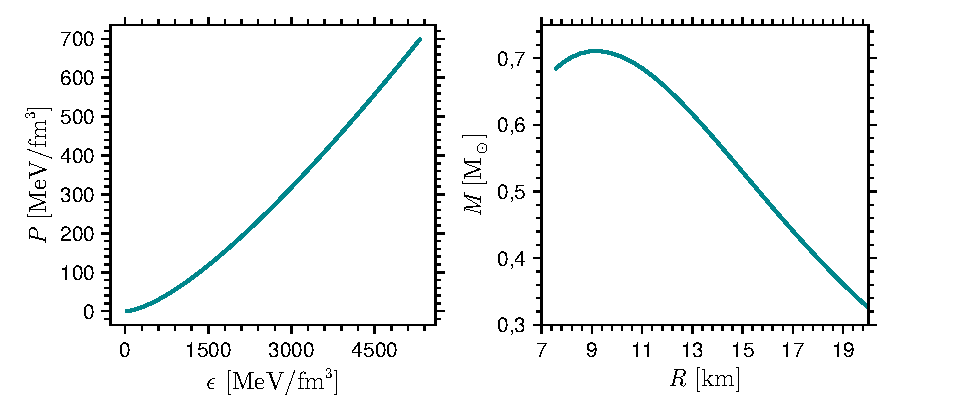
\includegraphics[width=0.9\textwidth]{eos_mr_fermigas.eps}
		\caption{Diagrama massa-raio gerado pela equação de estado de gás de Fermi.}
	\end{figure}
\end{frame}

\begin{frame}{Parametrização da EoS}
	\begin{itemize}
		\item Queremos encontrar uma forma da equação de estado que seja mais independente do modelo utilizado;
	\end{itemize}

	Uma forma paramétrica interessante é a que utiliza a velocidade do som definida por

	\begin{equation}
		c_s^2 = \left( \frac{\partial p}{\partial \epsilon} \right)_S.
	\end{equation}

	Dividindo o intervalo de densidade de energia em 5 segmentos uniformemente espaçados no logaritmo no intervalo $(\epsilon_0,8\epsilon_0]$ ($\epsilon_0 = 150$ MeV fm$^{-3}$) podemos obter as pressões e densidades de energia nas interfaces desses segmentos a partir da velocidade do som média no intervalo\footfullcite{Fujimoto_2021}.

	\begin{equation}
		p_i = p_{i-1} + c_{s,i}^2 (\epsilon_i - \epsilon_{i-1}).
	\end{equation}
\end{frame}

\begin{frame}
	Utilizamos uma interpolação politrópica em que, no intervalo $i$ a pressão é dada por parâmetros $K_i$ e $\Gamma_i$

	\begin{equation}
		p = K_i \epsilon^{\Gamma_i}.
	\end{equation}

	\begin{block}{Resumindo:}
		\begin{itemize}
			\item Podemos obter o diagrama massa-raio a partir da equação de estado utilizando as equações de TOV;
			\item A EoS pode ser aproximada por uma forma paramétrica. Aqui utiliza-se a velocidade do som média em intervalos de densidade de energia;
			\item Essa forma paramétrica depende de uma equação de estado inicial (crosta), aqui é utilizada a SLy4\footnotemark;
		\end{itemize}
	\end{block}

	\footnotetext{\fullcite{Douchin_2001}.}
\end{frame}

\section{Machine learning}
\begin{frame}{Machine learning}
	\begin{itemize}
		\huge
		\item Aprendizado de máquina;
	\end{itemize}

	\vspace{0.5cm}

	Tendo uma forma paramétrica da equação de estado, podemos nos voltar ao problema de encontrar os parâmetros $\bm{c_s^2}$ que melhor ajustam os dados observacionais. Focaremos em duas abordagens:

	\begin{itemize}
		\item Análise Bayesiana;
		\item Redes neurais;
	\end{itemize}
\end{frame}

\begin{frame}{Análise Bayesiana}
	Utilizamos o teorema de Bayes

	\begin{equation}
		P(\bm c_s^2, \bm p_c | \bm D, I) \propto P(\bm D | \bm c_s^2, \bm p_c, I) P(\bm c_s^2, \bm p_c | I),
	\end{equation}
	em que as pressões centrais das estrelas de cada dado observacional foram adicionadas para a definição da \textit{likelihood}. Ainda, assumimos independência dos dados e \textit{priors}

	\begin{equation}
		\begin{aligned}
			P(\bm D | \bm c_s^2, \bm p_c, I) & = \prod_{k=1}^N P(D_k | \bm c_s^2, p_{c,k}, I),                                              \\
			P(\bm c_s^2, \bm p_c | I)        & = \left[ \prod_{i=1}^{n} P(c_{s,i}^2 | I)\right]\left[ \prod_{k=1}^N P(p_{c,k} | I) \right].
		\end{aligned}
	\end{equation}
\end{frame}

\begin{frame}
	Por fim, utilizamos \textit{likelihoods} gaussianas

	\begin{equation}
		\begin{aligned}
			P(\bm D | \bm c_s^2, \bm p_c, I) & \propto \exp\left( -\frac{\chi^2}{2} \right),                                                                                                      \\
			\chi^2                           & = \sum_{k = 1}^{N} \frac{[M(\bm c_s^2, p_{c,k}) - M_k]^2}{\sigma_{M,k}^2} + \sum_{k = 1}^N \frac{[R(\bm c_s^2, p_{c,k}) - R_k]^2}{\sigma_{R,k}^2}.
		\end{aligned}
	\end{equation}

	Os dados observacionais são ajustados por distribuições gaussianas com parâmetros $\{ R_k, M_k, \sigma_{R,k}, \sigma_{M,k} \}$ e então é utilizado um \textit{sampler} que retirará amostras da distribuição posterior $P(\bm c_s^2, \bm p_c | \bm D, I)$.
\end{frame}

\begin{frame}
	\begin{itemize}
		\item Intervalos de credibilidade e convenções desse trabalho;
	\end{itemize}

	\begin{figure}
		\centering
		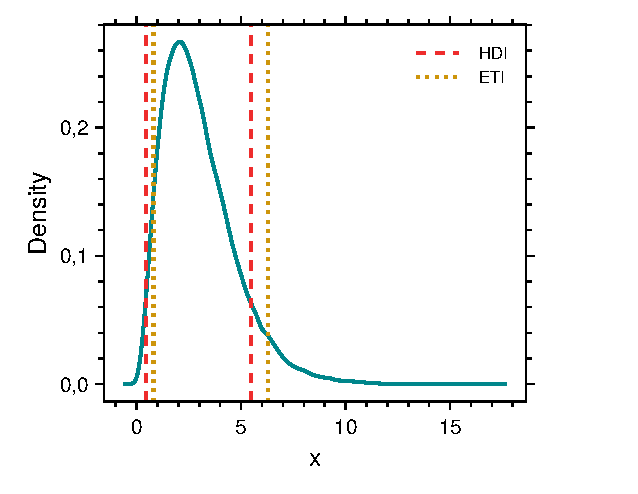
\includegraphics[width=0.7\textwidth]{hdi_eti_example.eps}
	\end{figure}
\end{frame}

\begin{frame}
	\begin{block}{Faz parte da análise}
		\begin{itemize}
			\item Parametrização utilizada;
			\item Escolha dos \textit{likelihoods};
			\item \textit{Priors};
			\item Algoritmo de amostragem, \textit{sampler};
		\end{itemize}
	\end{block}
\end{frame}

\begin{frame}{Redes neurais}
	\begin{itemize}
		\item Teorema de aproximação universal;
		\item Redes neurais profundas (DNNs);
	\end{itemize}

	\begin{minipage}{1.0\textwidth}
		\begin{minipage}{0.5\textwidth}
			O \textit{output} de uma unidade de uma DNN é dado por

			\begin{equation}
				a_j^l = \sigma\left(\sum_k w_{jk}^l a_k^{l-1} + b_j^l\right) = \sigma(z_j^l).
			\end{equation}
		\end{minipage}
		\begin{minipage}{0.5\textwidth}
			\begin{figure}
				\centering
				\includegraphics[width=1.0\textwidth]{neuralnetwork_representation.png}
				\caption{Representação de uma DNN.}
			\end{figure}
		\end{minipage}
	\end{minipage}
\end{frame}

\begin{frame}
	\begin{itemize}
		\item O teorema de aproximação universal não nos dá a arquitetura necessária (número de camadas, por exemplo) para aproximar uma função;
		\item Encontramos os parâmetros da rede utilizando um algoritmo de otimização de modo a minimizar uma função de erro;
		\item Para isso são necessários dados de treino que em alguns problemas podem ser gerados;
	\end{itemize}

	\vspace{0.5cm}

	A prática geral é gerar (ou extrair) um conjunto de dados $\{\bm x_j, \bm y_k\}$ e separar em duas partes: treino ($\sim 80 \%$) e validação ($\sim 20 \%$). Então temos a atualização dos parâmetros

	\begin{equation}
		\bm \theta_{i+1} = \bm \theta_i - \eta \bm \nabla_{\bm \theta} E(\bm \theta).
	\end{equation}
\end{frame}

\begin{frame}
	Alternativamente, isso é feito em \textit{minibatches}

	\begin{equation}
		\bm \theta_{i+1,k} = \bm \theta_{i,k} - \eta \bm \nabla_{\bm \theta} E_k(\bm \theta), \quad k = 1, \ldots, n/M.
	\end{equation}

	\begin{block}{Todos os seguintes são ajustáveis:}
		\begin{itemize}
			\item Número de camadas e unidades por camada;
			\item Funções de ativação;
			\item Tamanho do \textit{minibatch} $M$;
			\item Taxa de aprendizado $\eta$;
			\item Função de erro $E(\bm \theta)$;
			\item Algoritmo de otimização;
			\item Número de épocas;
		\end{itemize}
	\end{block}
\end{frame}

\section{Resultados}
\begin{frame}{Resultados da análise Bayesiana}

	\begin{itemize}
		\item Priors uniformes: $c_{s,i}^2 \sim \mathcal{U}(0, 1)$, $\epsilon_{c,i} \sim \mathcal{U}(0, 1)$;
	\end{itemize}

	Testamos as seguintes \textit{likelihoods}:

	\begin{equation}
		\begin{aligned}
			\mathcal{L}_\text{G}   & \propto \prod_i \exp\left( -\frac{1}{2} \left[ \frac{(M_i - \mu_{M,i})^2}{\sigma_{M,i}^2} + \frac{(R_i - \mu_{R,i})^2}{\sigma_{R,i}^2} \right] \right), \\
			\mathcal{L}_\text{GM}  & \propto \prod_i \exp\left( -\frac{1}{2} (\mathbf{x}_i - \mathbf{\mu}_i)^\text{T} \sigma_i^{-1} (\mathbf{x}_i - \mathbf{\mu}_i) \right),                 \\
			\mathcal{L}_\text{KDE} & \propto \sum_i K(\mathbf{x} - \mathbf{x}_i),
		\end{aligned}
	\end{equation}
	onde $\mathbf{x}_i = (M_i, R_i)$ e $\mathbf{\mu}_i = (\mu_{M,i}, \mu_{R,i})$.

\end{frame}

\begin{frame}
	\begin{figure}
		\centering
		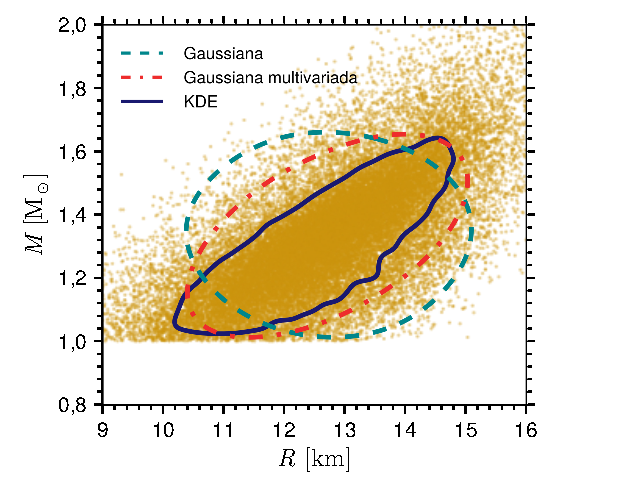
\includegraphics[width=0.7\textwidth]{likelihood_choice.eps}
	\end{figure}
\end{frame}



\section{Conclusão e perspectivas}
\begin{frame}{Conclusão e perspectivas}
\end{frame}

\begin{frame}{Agradecimentos}
	\centering
	\vspace*{\fill}
	\includegraphics[width=0.3\textwidth]{logo_fapergs.png}
	\includegraphics[width=0.2\textwidth]{logo_simee.png}
	\hspace{12pt}
	\includegraphics[width=0.3\textwidth]{logo_pet-cropped.jpg}

	\vspace{16pt}
	\includegraphics[width=0.2\textwidth]{logo-inct-fna.png}
	\hspace{24pt}
	\includegraphics[width=0.2\textwidth]{cnpq-eps-converted-to.pdf}

	\vspace*{\fill}
\end{frame}

\begin{frame}[allowframebreaks]{Referências}
	\footnotesize
	% \nocite{Raithel_2016,Fujimoto_2018}
	\printbibliography
\end{frame}

\begin{frame}[noframenumbering]{Massa máxima de estrelas de nêutrons}
	\begin{figure}
		\centering
		\includegraphics[width=0.5\textwidth]{maxmass.png}
		\caption{Ilustração de equilíbrio estável. Reproduzida de \fullcite{Glendenning}.}
	\end{figure}
\end{frame}

\begin{frame}[noframenumbering]{Markov Chain Monte Carlo}
	\begin{figure}
		\centering
		\includegraphics[width=0.75\textwidth]{mcmc.png}
	\end{figure}
\end{frame}

\begin{frame}[noframenumbering]
	Distribuição desejada $P(x)$ e a distribuição estacionária (processo de Markov) $\pi(x)$. Do teorema de Bayes

	\begin{equation}
		P(x) = P(x | D) = \frac{P(D | x) P(x)}{P(D)} = K f(x).
	\end{equation}

	Exigimos um processo detalhado no equilíbrio

	\begin{equation}
		P(x' | x)P(x) = P(x | x')P(x'),
	\end{equation}
	que temporariamente não vai ser satisfeito com
	\begin{equation}
		P(x' | x)P(x) > P(x | x')P(x'),
	\end{equation}
	estão acontecendo mais transições $x \to x'$.
\end{frame}

\begin{frame}[noframenumbering]
	Podemos separar a probabilidade de transição em duas partes

	\begin{equation}
		g(x' | x) \alpha(x' | x) P(x) > g(x | x') \alpha(x | x') P(x'),
	\end{equation}
	se queremos que esse equilíbrio aconteça, podemos maximizar o lado direito escolhendo $\alpha(x | x') = 1$ (estamos deixando todos as transições $x' \to x$ acontecer). Então impomos novamente o equilíbrio

	\begin{equation}
		\alpha(x' | x) = \frac{P(x) g(x | x')}{P(x') g(x' | x)},
	\end{equation}

	Esse expressão ainda pode ser maior que 1 (caso em que acontecem mais transições $x \to x'$), finalmente chegamos à \textit{acceptance function} de Metropolis

	\begin{equation}
		\alpha(x' | x) = \min\left(1, \frac{P(x) g(x | x')}{P(x') g(x' | x)}\right).
	\end{equation}
\end{frame}

\begin{frame}[noframenumbering]
	Algorítmo:

	\begin{enumerate}
		\item Escolha um ponto inicial $x_0$;
		\item Gere um candidato $x'$ a partir de uma distribuição $g(x' | x_i)$;
		\item Calcule a taxa de aceitação $\alpha(x' | x_i)$;
		\item Gere um número aleatório $u$ uniformemente distribuído em $[0,1]$;
		\item Se $u < \alpha(x' | x_i)$ aceite o candidato e defina $x_{i+1} = x'$, caso contrário rejeite o candidato e defina $x_{i+1} = x_i$;
	\end{enumerate}
\end{frame}

\begin{frame}[noframenumbering]{Problema de sinal}
	Em LQCD geralmente são calculados valores médios utilizando integrais de caminho da forma

	\begin{equation}
		\langle A \rangle_\rho = \frac{\int \mathcal{D}\sigma A[\sigma] \rho[\sigma]}{\int \mathcal{D}\sigma \rho[\sigma]},
	\end{equation}
	quando a parte fermiônica já é integrada analiticamente
	\begin{equation}
		\rho = \det M[\sigma] e^{-S[\sigma]},
	\end{equation}
	e temos algo do tipo
	\begin{equation}
		M = \slashed{D} + m + \mu \gamma^0.
	\end{equation}
\end{frame}

\begin{frame}[noframenumbering]
	O operador $\slashed{D}$ satisfaz

	\begin{equation}
		\gamma_5 \slashed{D} \gamma_5 = \slashed{D}^\dagger,
	\end{equation}
	enquanto que $\gamma_5 \gamma^0 \gamma_5 = -\gamma^0$. Então
	\begin{equation}
		\det(\slashed{D} + m + \mu \gamma^0) = \det(\slashed{D} + m - \mu^* \gamma^0)^\dagger,
	\end{equation}
	ou seja, para termos um determinante real precisamos de $\mu$ zero ou puramente imaginário\footfullcite{deForcrand_2009}.
\end{frame}

\begin{frame}[noframenumbering]
	Voltando ao valor médio, precisamos ter um determinante real e positivo para podermos utilizar o método de Monte Carlo utilizado para calcular as integrais de caminho com dimensionalidade muito alta. Temos algo do tipo

	\begin{equation}
		\int \mathcal{D}\sigma e^{-S} \sim \int d\sigma_1 d\sigma_2 \ldots d\sigma_N e^{-S}.
	\end{equation}

	Podemos reescrever integrais difíceis como valores médios utilizando uma distribuição uniforme\footfullcite{Gattringer_2010}

	\begin{equation}
		\frac{1}{b - a} \int_a^b dx f(x) = \langle f \rangle_\rho = \lim_{N \to \infty} \frac{1}{N} \sum_{i = 1}^N f(x_i),
	\end{equation}
	em que $x_i$ são amostras retiradas da distribuição uniforme $\rho(x) = 1/(b-a)$.
\end{frame}

\begin{frame}[noframenumbering]
	Porém, pontos que não contribuem tanto ainda são amostrados e com a mesma importância, aumentando bastante a variância do resultado. Vemos que no caso da integral de caminho o fator $e^{-S}$ da importância diferente para diferentes configurações de campo. Podemos fazer uma amostragem com \textit{importance sampling}, considere

	\begin{equation}
		\langle f \rangle_\rho = \frac{\int_a^b dx \; f(x) \rho(x)}{\int_a^b dx \rho(x)} = \lim_{N \to \infty} \frac{1}{N} \sum_{i=1}^N f(x_i),
	\end{equation}
	em que $x_i$ agora são amostrados de acordo com a probabilidade
	\begin{equation}
		dP(x) = \frac{\rho(x) dx}{\int_a^b dx \rho(x)}.
	\end{equation}
\end{frame}

\begin{frame}[noframenumbering]
	Em particular

	\begin{equation}
		\langle A \rangle = \lim_{N \to \infty} \frac{1}{N} \sum_{i=1}^N A[\sigma_n],
	\end{equation}
	em que as configurações de campo $U_n$ são amostradas de acordo com a probabilidade
	\begin{equation}
		dP[\sigma] = \frac{e^{-S[\sigma]} \mathcal{D}\sigma}{\int \mathcal{D}\sigma e^{-S[\sigma]}}.
	\end{equation}
\end{frame}

\begin{frame}[noframenumbering]
	\begin{figure}
		\centering
		\includegraphics[width=0.5\textwidth]{oscillatory_2d3.eps}
		\caption{Integração de uma função oscilatória $f(x) = \exp(-x^2 + i \lambda x)$. Imagem de \fullcite{deForcrand_2009}}
	\end{figure}
\end{frame}

\end{document}
